\documentclass[a4j,11pt]{jarticle}
%\usepackage[dviout]{graphicx}
%\usepackage[dvipdfm]{graphicx}
\usepackage[dvipdfmx]{graphicx}
\usepackage{amsmath}
\usepackage{amssymb}
\usepackage{ascmac}
%\usepackage{epsbox}
\usepackage{float}
\usepackage{here}
\usepackage{lscape}
\usepackage{latexsym}
\usepackage{pifont}
\usepackage{wrapfig}
\usepackage{type1cm}
\usepackage{algorithm}
\usepackage{algorithmic}
\usepackage{txfonts}
\usepackage{bm}
\usepackage{comment}
\usepackage{url}
\usepackage[round]{natbib}

\usepackage{listings}
%\usepackage{plistings}

%\setlength{\voffset}{-25.4mm}
\setlength{\topmargin}{-17.5mm}   %トップとヘッダの間隔
%\setlength{\headheight}{20mm}   %ヘッダの高さ
%\setlength{\headsep}{0mm}   %ヘッダとテキストの間隔
\setlength{\textwidth}{45zw}   %テキストの幅
\setlength{\hoffset}{-10mm}
\setlength{\textheight}{45\baselineskip}   %テキストの高さ
%\addtolength{\textheight}{\topskip}
%\setlength{\footskip}{0mm}
%\setlength{\oddsidemargin}{21.5mm}   %サイドとテキストの間隔(奇数ページ)
%\setlength{\evensidemargin}{21.5mm}   %サイドとテキストの間隔(偶数ページ)
\pagestyle{empty}   %ページ番号なし
\newcommand{\g}[1]{\boldsymbol{#1}}
\newcommand{\lw}[1]{\smash{\lower2.0ex\hbox{#1}}}
\renewcommand{\baselinestretch}{1.0}

\makeatletter
%\def\theequation{\arabic{equation}}   %数式番号を(章.式)形式
%\@addtoreset{equation}{section}
%\def\thefigure{\thesection.\arabic{figure}}   %図番号を(章.図)形式
%\@addtoreset{figure}{section}
%\def\thetable{\thesection.\arabic{table}}   %表番号を(章.表)形式
%\@addtoreset{table}{section}
\def\tr{\mathop{\operator@font tr}\nolimits}
\def\grad{\mathop{\operator@font grad}\nolimits}
\def\St{\mathop{\operator@font St}\nolimits}
\def\Hess{\mathop{\operator@font Hess}\nolimits}
\def\D{\mathop{\operator@font D}\nolimits}
\def\sym{\mathop{\operator@font sym}\nolimits}
\def\s.t.{\mathop{\operator@font s.t.}\nolimits}
\def\diag{\mathop{\operator@font diag}\nolimits}
\def\section{\@startsection{section}{1}{\z@}
   {0.8\Cvs \@plus.5\Cdp \@minus.2\Cdp}
   {0.2\Cvs \@plus.3\Cdp}
   {\normalfont \Large \bfseries}}
\makeatother
\makeatletter
\def\subsection{\@startsection{subsection}{1}{\z@}
   {0.8\Cvs \@plus.5\Cdp \@minus.2\Cdp}
   {0.2\Cvs \@plus.3\Cdp}
   {\normalfont \normalsize \bfseries}}
\makeatother
\makeatletter
\newcommand{\figcaption}[1]{\def\@captype{figure}\caption{#1}}
\newcommand{\tblcaption}[1]{\def\@captype{table}\caption{#1}}
\makeatother

% 参考文献の間隔調整
\makeatletter
\renewenvironment{thebibliography}[1]
{\section*{\refname\@mkboth{\refname}{\refname}}%
   \list{\@biblabel{\@arabic\c@enumiv}}%
        {\settowidth\labelwidth{\@biblabel{#1}}%
         \leftmargin\labelwidth
         \advance\leftmargin\labelsep
	 \setlength\itemsep{-0.3zh}%←ここの数値を調整
         \@openbib@code
         \usecounter{enumiv}%
         \let\p@enumiv\@empty
         \renewcommand\theenumiv{\@arabic\c@enumiv}}%
   \sloppy
   \clubpenalty4000
   \@clubpenalty\clubpenalty
   \widowpenalty4000%
   \sfcode`\.\@m}
  {\def\@noitemerr
    {\@latex@warning{Empty `thebibliography' environment}}%
   \endlist}

\def\JTeX{\leavevmode\lower .5ex\hbox{J}\kern-.17em\TeX}
\def\JLaTeX{\leavevmode\lower.5ex\hbox{J}\kern-.17em\LaTeX}

\makeatother

\begin{document}
\bibliographystyle{plainnat}
%\bibliographystyle{aer2} %参考文献に番号ふらない
%\bibliographystyle{ecta} %参考文献に番号ふらない
%\bibliographystyle{apalike} %いらない

\begin{center}
{\Large \textbf{混合射影正規分布によるクラスタリングについて}}
\end{center}
\begin{flushright}
小坪 琢人(塩濱 敬之准教授)
\end{flushright}
\vspace{-3zh}

%%%%%%%%%%%%% これ以下, 本文 %%%%%%%%%%%5%%
%%%%%%%%%%%%%  section1  はじめに %%%%%%%%%%%%%%%

\section{はじめに}

円周上や球面上のデータを扱う統計手法を方向統計学といい, 近年多様体上の統計分析手法として, 注目を集めている. 方向統計学とは風向データ, 渡り鳥の移動方向データなどの角度観測値を含むデータを対称とする統計学である. 単位超球面上 $(\mathbb{S}^{p-1})$ に分布するようなデータをユークリッド空間上のデータとして扱うと不適当なことがある. データを多様体上の分布として扱うことで, 数学的モデルを作る際に低次元で考えられるなどの利点がある. 円周あるいは超球面上の分布を生成するいくつかの方法が知られている. 代表的なものは, 巻き込み法, 射影法, 条件付法, 投影法である. 本研究では射影法を用いた射影分布によるクラスタリングについて議論する.

代表的なクラスタリング手法として, $k$平均法が挙げられる. $k$平均法は, 各データと各クラスタの中心のユークリッド距離を最小化することで, 各データをクラスタリングする. しかし確率変数が円周上や球面上に値をとるようなデータに対して, ユークリッド空間のクラスタリングを前提とした$k$平均法はしばしば誤った分類結果をもたらす. \citet{SKMcluster}は, ユークリッド距離に基づく非類似度の尺度を単位球面上に射影したコサイン非類似度の最小化に基づく超球面上の$k$平均法を提案した. データの単位方向ベクトルと各クラスタにおける重心ベクトルとのコサイン非類似度を最小化することで, 各データをクラスタリングする. 

超球面上の$k$平均法は確率モデルを仮定しないノンパラメトリックな手法であるのに対し,  パラメトリックな超球面上のクラスタリング手法として, \citet{Gopal}による von Mises Fisher 分布の混合分布を用いた手法がある. 単位超球面上の分布として知られる, von Mises Fisher 分布を用いて, MCMCサンプリングにより高次元データのクラスタリングを行う. MCMCを用いることで求める事後分布のパラメータの平均値, 標準偏差を求めることができる. 本研究では方向データの分布として知られる, 射影正規分布の混合分布によるクラスタリングの性能評価を行う. 

%%%%%%%%%%%%%%%%%%%%%%%% senction2 混合分布 %%%%%%%%%%%%%%%%%%%%%
\vspace{-1zh}
\section{混合射影正規分布}
\vspace{-0.5zh}
\subsection{射影正規分布}

射影分布は平面または空間上の放射状の射影によって得られる. 一般的には, 多変量正規ベクトルをノルムで割ることで, 単位超球面上への射影分布が得られる. 多変量正規ベクトル($k$次元)を$X$として, $k \geq 2$ の場合には, 単位超球面上への単位ベクトル $U$ は $U = X/||X||$ で表される. このとき$U$は$k$次元の一般化射影正規分布に従い, $U \sim \mathcal{PN}_k(\bm \mu,\Sigma)$と表せる. 一般化射影正規分布は, パラメータ$\bm \mu, \Sigma$をもち, \citet{PML}で, $\Sigma = \mathcal{I}$と定義されていた射影正規分布を一般化したものである. $\mathcal{PN}_k(\bm \mu,\mathcal{I})$は平均方向$\bm \mu$に対して, 単峰性かつ対称の分布となるが, $\mathcal{PN}_k(\bm \mu,\Sigma)$では非対称分布もしくは二峰性分布となる. ここで平均方向について説明する. $\pi/3$ ラジアンと$5\pi/3$ ラジアン の平均方向について考える. 算術平均では$(\pi/3 + 5\pi/3)/2 = \pi$ となるが, 2つの平均方向としては不適切なことが分かる. よってこれらの角度を円周上の点 $(\cos \frac{\pi}{3},\sin \frac{\pi}{3}) = (\frac{1}{2},\frac{\sqrt{3}}{2}),\ (\cos \frac{5\pi}{3}, \sin \frac{5\pi}{3}) = (\frac{1}{2},- \frac{\sqrt{3}}{2})$ と表し, 2つのベクトルの平均を取ることで $\frac{1}{2} (\cos 0, \sin 0)$ となり, 平均方向は$0$ラジアンとなる. 

\citet{PN1}によると, $\mathcal{PN}_2(\bm \mu,\Sigma$)の円形データの場合, 単位円上の方向を表す$U = (\cos\Theta, \sin\Theta)^T$における$\theta$の確率密度を式(\ref{PNC})に示す.

\vspace{-1.5zh}
\begin{eqnarray}
\label{PNC}
p(\theta; \bm \mu, \Sigma) = \frac{1}{2\pi A(\theta)}|\Sigma|^{-\frac{1}{2}}
\exp(C)\left\{1 + \frac{B(\theta)}{\sqrt{A(\theta)}} \frac{\Phi \left(\frac{B(\theta)}{\sqrt{A(\theta)}}\right)}{\phi \left(\frac{B(\theta)}{\sqrt{A(\theta)}}\right)}\right\} I_{[0,2\pi)}(\theta),
\end{eqnarray}

\noindent
ここで, $\bm u^T = (\cos\theta,\sin\theta), \ A(\theta) = \bm u^T\Sigma^{-1}\bm u, \ B(\theta) = \bm u^T \Sigma^{-1} \bm \mu, \ C = -\frac{1}{2} \bm \mu^T \Sigma^{-1} \bm \mu$であり, $I_{[0,2\pi)} (\cdot)$は指示関数, $\Phi(\cdot), \phi(\cdot)$ は標準正規分布の確率密度関数と累積密度関数である.

射影正規分布において対称分布, 非対称分布, 二峰性分布となる例を図$\ref{sample_pn}$に示す. 

\vspace{-0.5zh}
\begin{figure}[H]
 \begin{tabular}{c}
\hspace{0.5cm}
 \begin{minipage}{0.33\hsize}
  \begin{center}
   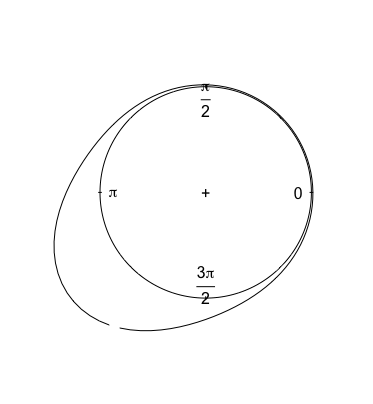
\includegraphics[clip,height= 40mm]{data/sample_symmetry.png}
  \end{center}
 \end{minipage}
\hspace{-1.0cm}
 \begin{minipage}{0.33\hsize}
  \begin{center}
 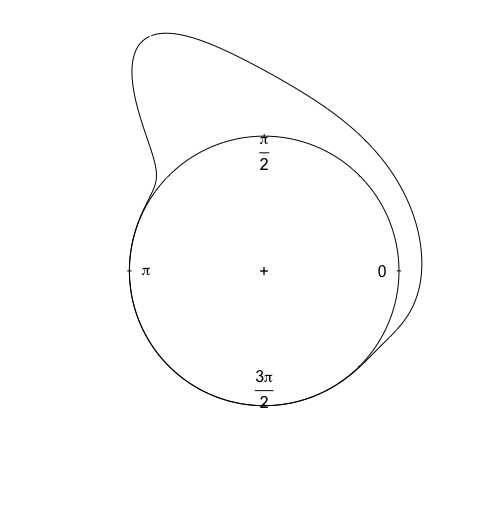
\includegraphics[clip,height= 40mm]{data/sample_asymmetry.png}
  \end{center}
 \end{minipage}
\hspace{-1.0cm}
 \begin{minipage}{0.33\hsize}
  \begin{center}
   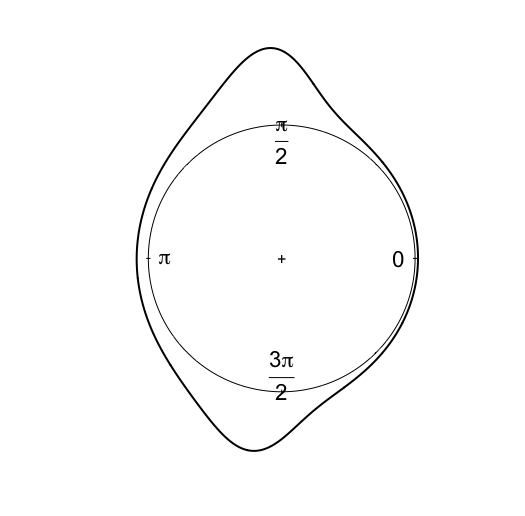
\includegraphics[clip,height= 40mm]{data/sample_bimodal.png}
  \end{center}
 \end{minipage}
  \end{tabular}
\vspace{-0.5zh}
\caption[Text excluding the matrix]{
$\bm \mu = \begin{pmatrix} -1.2 \\ -0.95 \\ \end{pmatrix}, \ \Sigma = \begin{pmatrix}  1 & 0 \\ 0 & 1 \\ \end{pmatrix}$
とした場合の対称な射影正規分布(左), 
\ $\bm \mu = \begin{pmatrix} -0.19 \\ 2.09 \\ \end{pmatrix}, \ \Sigma = \begin{pmatrix} 2.49 & -1.85 \\ -1.85 & 1.96 \\ \end{pmatrix}$ とした場合の非対称な射影正規分布(中央), 
\ $\bm \mu = \begin{pmatrix} -0.24 \\ 0.15 \\ \end{pmatrix}, \ \Sigma = \begin{pmatrix} 0.209 & 0.068\\ 0.068 & 2.25 \\ \end{pmatrix}$ とした場合の二峰性となる射影正規分布(右).}
\label{sample_pn}
\end{figure}
\if0
\vspace{-0.5zh}
\begin{figure}[H]
 \begin{tabular}{c}
\hspace{0.5cm}
 \begin{minipage}{0.33\hsize}
  \begin{center}
   \includegraphics[height= 40mm]{data/Rplot3.eps}
  \end{center}
 \end{minipage}
\hspace{-1.0cm}
 \begin{minipage}{0.33\hsize}
  \begin{center}
 \includegraphics[height= 40mm]{data/Rplot1.eps}
  \end{center}
 \end{minipage}
\hspace{-1.0cm}
 \begin{minipage}{0.33\hsize}
  \begin{center}
   \includegraphics[height= 40mm]{data/Rplot2.eps}
  \end{center}
 \end{minipage}
  \end{tabular}
\caption[Text excluding the matrix]{
$\bm \mu = \begin{pmatrix} -1.2 \\ -0.95 \\ \end{pmatrix}, \ \Sigma = \begin{pmatrix}  1 & 0 \\ 0 & 1 \\ \end{pmatrix}$
とした場合の対称な射影正規分布(左), 
\ $\bm \mu = \begin{pmatrix} -0.19 \\ 2.09 \\ \end{pmatrix}, \ \Sigma = \begin{pmatrix} 2.49 & -1.85 \\ -1.85 & 1.96 \\ \end{pmatrix}$ とした場合の非対称な射影正規分布(中央), 
\ $\bm \mu = \begin{pmatrix} -0.24 \\ 0.15 \\ \end{pmatrix}, \ \Sigma = \begin{pmatrix} 0.209 & 0.068\\ 0.068 & 2.25 \\ \end{pmatrix}$ とした場合の二峰性となる射影正規分布(右)}
\label{sample_pn}
\end{figure}
\fi

% Wang and Gelfand(2013) によると各パラメータの単一の影響は良く分かっていない. だから各パラメータを細かく説明するのは困難である. しかしこの分布の柔軟な特性は予測などにおいて便利である.

\citet{GPN}によると, $\mathcal{PN}_3(\bm \mu,\Sigma$)の球形データの場合, 単位球面上の方向を表す$U = (\cos\Theta_1 \sin \Theta_2, \sin\Theta_1 \sin \Theta_2, \cos \Theta_2)^T$における$\bm \theta = (\theta_1, \theta_2)^T$の確率密度を式(\ref{PNS})に示す.

\vspace{-1zh}
\begin{eqnarray}
\label{PNS}
p(\bm \theta; \bm \mu, \Sigma) = \left(\frac{1}{2\pi A(\bm \theta)}\right)^{\frac{3}{2}} |\Sigma|^{-\frac{1}{2}}
\exp(C)\left( \left[1 + D(\bm \theta) \frac{\Phi \{D(\bm \theta)\}}{\phi \{D(\bm \theta)\}} \right] D(\bm \theta) + \frac{\Phi \{D(\bm \theta)\}}{\phi \{D(\bm \theta)\}} \right) I_{[0,2\pi)}(\theta_1) I_{[0,\pi)}(\theta_2).
\end{eqnarray}

\noindent
ここで, $\bm u^T = (\cos\theta_1 \sin \theta_2, \sin\theta_1 \sin \theta_2, \cos \theta_2), 
\ D(\bm \theta) = B(\bm \theta) A^{-\frac{1}{2}}(\bm \theta), \ A(\bm \theta) = \bm u^T \Sigma^{-1} \bm u, \ B(\bm \theta) = \bm u^T \Sigma^{-1} \bm \mu, \ C = -\frac{1}{2} \bm \mu^T \Sigma^{-1} \bm \mu$であり, $I_{[0,2\pi)} (\cdot), I_{[0,\pi)}(\cdot)$は指示関数, $\Phi(\cdot), \phi(\cdot)$ は標準正規分布の確率密度関数と累積密度関数である.

\vspace{-1zh}
\subsection{混合射影正規分布}

%%%%%%%%%%%%%%%%  球面 %%%%%%%%%%%%%%%%%%%%%%%%%%
$m$個のユニットからなる球面上の射影正規分布の混合分布を式(\ref{MPNS})に示す. 

\vspace{-2zh}
\begin{eqnarray}
\label{MPNS}
p(\bm \theta;\bm w,\bm \mu, \Sigma) = \sum^m_{j=1} w_j \mathcal{PN}_3(\bm \theta;\bm \mu_j, \Sigma_j),
\end{eqnarray}

\vspace{-1zh}
\noindent
ただし, $w_j$は混合比率であり, $0 < w_j < 1$, $\sum^m_{j=1} w_j = 1$を満たす. 混合射影正規分布におけるパラメータは, $w, \bm \mu_j, \Sigma_j$であるが, 球面上の混合射影正規分布のパラメータについては識別性を考慮して次のように分散共分散行列を定式化する. 

\vspace{-2zh}
\begin{eqnarray}
\label{SIGMA}
 \Sigma_j = \left(
    \begin{array}{cc}
      \Sigma^*_j + \bm \gamma_j \bm \gamma_j^T & \bm \gamma_j \\
      \bm \gamma_j^T & 1
    \end{array}
  \right),
\end{eqnarray}

\vspace{-0.5zh}
\noindent
と定義されるので, パラメータベクトルは$\bm \eta = (w_1, \dots, w_m, \bm \mu_1, \dots, \bm \mu_m, \Sigma^*_1, \dots, \Sigma^*_m, \bm \gamma_1, \dots, \bm \gamma_m)^T$となり, パラメータベクトルの次元は $d = 4m$ となる. ここで, 混合射影正規分布のパラメータのベイズ推定を考える. そのためにモデルパラメータの事前分布を定義する必要がある. 各パラメータの事前分布を $\bm \mu_j \sim N(\bm 0, 10^5 \bm I_3)$,\ $\bm \gamma_j \sim  N(\bm 0, 10^5 \bm I_2)$,\ $\Sigma^*_j \sim \mathrm{inverse Wishart}(4,\bm I_2)$,\ $\bm w \sim Dirichlet(2,2, \dots, 2)$ と設定する. ここで混合比率$\bm w$は$m$次の$Dirichlet$分布に従うものとする. $\bm \mu_j,\ \bm \gamma_j$は$0$付近に存在するという基準化したデータを想定した下で, 正規分布による弱情報事前分布とし, $\Sigma^*_j$は正定値対象行列となるように, 多変量正規分布の共分散行列の共役事前分布として扱われる逆ウィシャート分布を用いる. $\bm w$は非負かつ和が $1$となる性質をもつディリクレ分布を弱情報事前分布とする.

角度データ $\bm \theta$ が得られたときの, パラメータベクトル $\bm \eta$の事後分布を $p(\bm \eta| \bm \theta)$, パラメータベクトルの事前分布を $p(\bm \eta)$とすると事後分布を式(\ref{BAYES})に示す. 

\vspace{-1zh}
\begin{eqnarray}
\label{BAYES}
p(\bm \eta | \bm \theta) = \frac{p(\bm \theta | \bm \eta) p(\bm \eta)}{p(\bm \theta)} \propto p(\bm \theta | \bm \eta) p(\bm \eta)
\end{eqnarray}

\vspace{-0.5zh}
\noindent
すなわち, 事後分布$p(\bm \eta | \bm \theta)$は尤度$p(\bm \theta | \bm \eta)$と事前分布 $p(\bm \eta| \bm \theta)$の積に比例する. ここで, $p(\bm \theta)$はすでに得られた, データ$\bm \theta$にのみ依存する定数値であるので, $p(\bm \theta | \bm \eta) p(\bm \eta)$が $\bm \eta$  の事後分布の核関数を形成し, $p(\bm \theta)$は正規化定数とみなすことができる. 尤度と事前分布の計算は簡単だが, 周辺分布 $p(\bm \theta)$の計算は一般に簡単ではないので, 事後分布に比例する分布 $p(\bm \theta | \bm \eta) p(\bm \eta)$ から乱数サンプルを発生させる. この方法で得られたサンプルをMCMCサンプルと呼ぶ. %尤度関数を式$(\ref{logPNS})$に示す. 
\if0
\vspace{-1zh}
\begin{eqnarray}
\label{logPNS}
\log p(\bm \theta | \bm \eta) &=& \sum^m_{j=1} \{\log w_j + \log \mathcal{PN}_3(\bm \theta;\bm \mu_j, \Sigma_j)\} \nonumber \\ 
&=& \sum^m_{j=1} \left[ \log w_j - \frac{3}{2} \log 2\pi - \frac{3}{2} \log A - \frac{1}{2} \log |\Sigma_j| + C + \log \left( \left[1 + D(\bm \theta) \frac{\Phi \{D(\bm \theta)\}}{\phi \{D(\bm \theta)\}} \right] D(\bm \theta) + \frac{\Phi \{D(\bm \theta)\}}{\phi \{D(\bm \theta)\}} \right)\right] \nonumber \\
&\propto& \sum^m_{j=1} \left[ \log w_j - \frac{3}{2} \log A - \frac{1}{2} \log |\Sigma_j| + C + \log \left( \left[1 + D(\bm \theta) \frac{\Phi \{D(\bm \theta)\}}{\phi \{D(\bm \theta)\}} \right] D(\bm \theta) + \frac{\Phi \{D(\bm \theta)\}}{\phi \{D(\bm \theta)\}} \right) \right]  
\end{eqnarray}
\fi
%%%%%%%%%%%%%%%%%%%%%%%%%%%%%%%%%%%%%%%%%%%%%%%%%%%%%%%%%%%%%%%%%%%
%%%%%%%%%%%%%%%%%%%%%%%  sectio3 解析手法 %%%%%%%%%%%%%%%%%%%%%%%%
\vspace{-1zh}
\section{解析手法}
%\vspace{-0.5zh}
%\subsection{マルコフ連鎖モンテカルロ法}

本研究ではMCMCアルゴリズムの一つである, ハミルトニアン$\cdot$モンテカルロ法(HMC)を用いて分布の推定を行う. 
ハミルトニアンとはポテンシャルエネルギー $U(\bm \eta)$ と運動エネルギー $V(\bm q)$ の和で定義される物理量 $H(\bm \eta, \bm q) = U(\bm \eta) + V(\bm q)$ のことであり. ここで, $\bm q = (q_1, \dots, q_d)^T$ は$\bm \eta$ と同じ$d$次元のベクトルである. $t$番目のステップにおける, ハミルトニアン方程式は式$(\ref{HMC})$で定義される. 

\vspace{-1zh}
\begin{eqnarray}
\label{HMC}
\frac{d \eta_j(t)}{dt} = \frac{\partial V(\bm q)}{\partial q_j},\ \ \frac{d q_j(t)}{dt} = - \frac{\partial U(\bm \eta)}{\partial \eta_j},
\end{eqnarray}

\vspace{-0.5zh}
\noindent
ここで, $\bm \eta, \bm q$ の同時確率密度関数 $p(\bm \eta, \bm q)$ をハミルトニアン $H(\bm \eta, \bm q)$の関数で定義したとき, 上記のハミルトン方程式に従って, $\bm \eta, \bm q$の値を変化させると, 確率密度関数 $p(\bm \eta, \bm q) = f(H(\bm \eta, \bm q))$ からのサンプリングとみなすことができる. また$\bm \eta, \bm q$が独立であることを用いて, リープ$\cdot$フロッグ法で$\bm \eta$の分布を求める. 詳しい解説は\citet{HMC}を参照されたい.
%リープ$\cdot$フロッグ法について以下に簡単に示すが, 
\if0
\vspace{-1zh}
\begin{enumerate}

\item{}
$\eta_j(0), q_j(0)$の初期値を設定する. $\eta_j(0)$は各パラメータの事前分布からの設定し, $q_j(0)$は$N(0,M_j)$からランダムサンプリングする. $M_j$ は任意の分散パラメータである. 
 
\item{}
以下の式に従い, $\bm \eta, \bm q$を更新する. $\epsilon$は状態変化のステップ幅を表す.

\vspace{-2zh}
\begin{eqnarray*}
\label{leapflog}
q_j(t+\frac{\epsilon}{2}) = q_j(t) - \frac{\epsilon}{2} \frac{\partial U}{\partial \eta_j} (\bm \eta(t)),
\eta_j(t+\epsilon) = \eta_j(t) + \epsilon \frac{q_j(t + \frac{\epsilon}{2})}{M_j},
q_j(t+\epsilon) = q_j(t+\frac{\epsilon}{2}) - \frac{\epsilon}{2} \frac{\partial U}{\partial \eta_j} (\bm \eta(t + \epsilon))
\end{eqnarray*}

\item{}
得られたパラメータの採択, 棄却を決定する. 上記のステップで得られたパラメータを$\bm \eta^*, \bm q^*$として,
現在が$t$回目の反復とすると, サンプルの棄却率は

\vspace{-2zh}
\begin{eqnarray*}
\label{sampleget}
r = \frac{p(\bm \eta^*|\bm \theta) p(\bm q^*)}{p(\bm \eta(t-1)|\bm \theta) p(\bm q(t-1))}
\end{eqnarray*}

\noindent
\vspace{-1zh}
と定義する. 一様乱数 $u \sim U(0,1)$を発生し, $r > u$ならば, ランダムサンプル $\bm \eta^*$を採択する. 

\end{enumerate}
\fi
%%%%%%%%%%%%%%%%%%%%%%%%%%%%%%%%%%%%%%%%%%%%%%%%%%%%%%%%%%%%%%%%%%%
%%%%%%%%%%%%%%%%%%%%%%%  sectio4 数値実験 %%%%%%%%%%%%%%%%%%%%%%%%
\vspace{-0.5zh}
\section{データ解析}

\vspace{-0.5zh}
\subsection{評価指標}

情報量基準(WAIC)を用いて, 混合分布のコンポーネントの選択を行う. AICやBICなどの情報量基準には, 事後分布が正規分布で近似されている必要があるなど, 様々な制約が存在するが, WAICは真の分布, 確率モデル, 事前分布がどのような場合でも用いることができる. WAICは式$(\ref{WAIC1})$で求められる.

\vspace{-1zh}
\begin{eqnarray}
\label{WAIC1}
\mbox{WAIC} = T + \frac{V}{n}
\end{eqnarray}

\vspace{-0.5zh}
\noindent
ここで, $T = - \frac{1}{n} \Sigma^n_{i=1} \log E_{\bm \eta}[p(\bm \theta_i| \bm \eta)], 
V = \Sigma^n_{i=1} \{ E_{\bm \eta}[(\log p(\bm \theta_i| \bm \eta))^2] - E_{\bm \eta}[\log p(\bm \theta_i| \bm \eta)]^2 \}$であり, $n$は$\bm \theta$のデータ数である. また$E_{\bm \eta}[ ]$は$\bm \eta$の事後分布の下で評価した期待値である.  

\vspace{-0.5zh}
\subsection{クラスター分析}

MovieLensのデータセットから, $943$人の$1682$個の映画へのレビューを用いる. レビューには$0\sim6$の値があり, $0$は見ていないことを表し, $1\sim5$は見た映画に対する評価値である. 数字が大きいほど高い評価値を表す. 映画に対する評価に基づいて, ユーザをクラスタリングする. このデータは$94\%$が$0$であるスパースな行列として表せる. 次元圧縮の手法として知られている\citet{tSNE}の t-SNEを用いてデータを3次元に圧縮する. 得られたデータを正規化し, 極座標変換することで角度データ$\bm \theta = (\theta_1, \theta_2)^T$を得る. t-SNEにより得られた異なる$10$個の$3$次元データに対し, クラスター数を$1$から$4$まで変化させた場合のWAICを表$\ref{WAIC}$に示す. 

\vspace{-1zh}
\begin{table}[H]
\caption{WAICによるコンポーネントの選択結果}
\label{WAIC}
\begin{center}
\scalebox{0.8}{
\begin{tabular}{l | c c c c c c c c c c}
\hline
 & 1 & 2 & 3 & 4 & 5 & 6 & 7 & 8 & 9 & 10 \\ \hline 
$m=1$ & -1014.1 & -1237.0 & -1350.6 & -1009.5 & -1308.8 & -1227.8 & -1152.4 & -902.5 & -1322.6 & -1140.2 \\ 
$m=2$ & -1610.9 & -1675.0 & -1760.4 & -1552.8 & -1633.1 & -1529.6 & -1507.1 & -1366.1 & -1645.2 & -1693.3 \\ 
$m=3$ & -1846.8 & -1744.7 & -1728.9 & -1804.9 & -1741.0 & -1654.3 & -1705.2 & -1633.8 & -1789.3 & \textbf{-1872.1} \\ 
$m=4$ & \textbf{-1893.6} & \textbf{-1969.8} & \textbf{-1901.6} & \textbf{-1837.5} & \textbf{-1787.5} & \textbf{-1687.8} &\textbf{-1749.5} & \textbf{-1686.7} & \textbf{-1844.5} & -1802.6 \\ 
\hline
\end{tabular}
}
\end{center}
\end{table}

\noindent
$9$個のデータにおいて, クラスター数が$4$つのときWAICが最小になっていることがわかる. クラスター数を$4$つとして混合射影正規分布によるクラスタリングを行う. HMCによって推定された混合射影正規分布のパラメータを式$(\ref{parameter})$に示す. なお, $\hat {\bm w}$はクラスターごとの混合比率を表し, パラメータの添え字はクラスターの番号に対応している.

\vspace{-1.5zh}
\begin{equation}
\label{parameter}
\begin{split}
\hat {\bm w} = \begin{pmatrix} 0.26 \\ 0.51 \\ 0.20 \\ 0.03 \\ \end{pmatrix},\ 
\hat{\bm \mu}_1 = \begin{pmatrix} 0.44 \\ 2.85 \\ -1.67 \\ \end{pmatrix},\ 
\hat \Sigma_1 = \begin{pmatrix}  2.40 & 1.52 &  0.06 \\ 1.52 & 2.20 & -0.25 \\ 0.06 & -0.25 &1.00 \\ \end{pmatrix},\ 
\hat{\bm \mu}_2 = \begin{pmatrix} 0.14 \\ -0.50 \\ 1.09 \\ \end{pmatrix},\ 
\hat \Sigma_2 = \begin{pmatrix}   0.28  & 0.14 &  0.20 \\ 0.14 & 0.61 & 0.06 \\  0.20 & 0.06 &1.00 \\ \end{pmatrix}, \\
\hat{\bm \mu}_3 = \begin{pmatrix} -2.08  \\ -1.96 \\ -8.11 \\ \end{pmatrix},\ 
\hat \Sigma_3 = \begin{pmatrix}  1.86  & -0.18 &  -0.10 \\-0.18 & 3.89 & 1.60 \\  -0.10 & 1.60 & 1.00 \\ \end{pmatrix},\ 
\hat{\bm \mu}_4 = \begin{pmatrix} -12.29   \\ -2.48 \\ -4.84 \\ \end{pmatrix},\ 
\hat \Sigma_4 = \begin{pmatrix} 15.19 & 4.01 &  0.12 \\ 4.01 & 1.88 & 0.08 \\ 0.12 & 0.08 &1.00 \\ \end{pmatrix}.
\end{split}
\end{equation}

%%%% どっちにしようか %%%%%%%%%
\if0
\begin{wrapfigure}[15]{r}[5mm]{70mm}
\vspace{-0.5cm}
\begin{center}
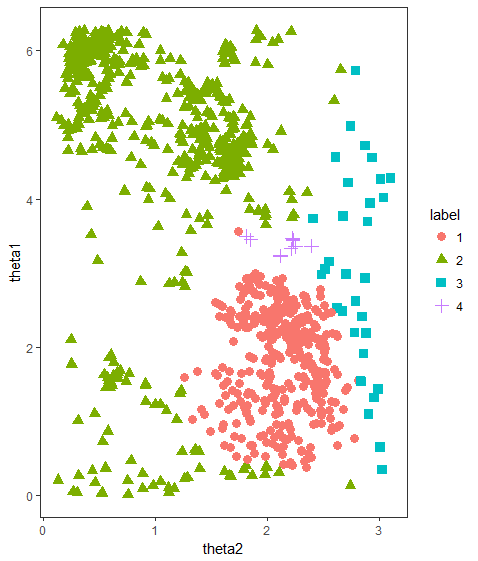
\includegraphics[clip,height= 70mm]{data/cluster_4.png}
\end{center}
 \vspace{-0.9cm}
\caption{クラスタリング結果}
\label{skmeans}
\end{wrapfigure}
\fi

\begin{wrapfigure}[17]{r}[-5mm]{70mm}
\vspace{-0.5cm}
\begin{center}
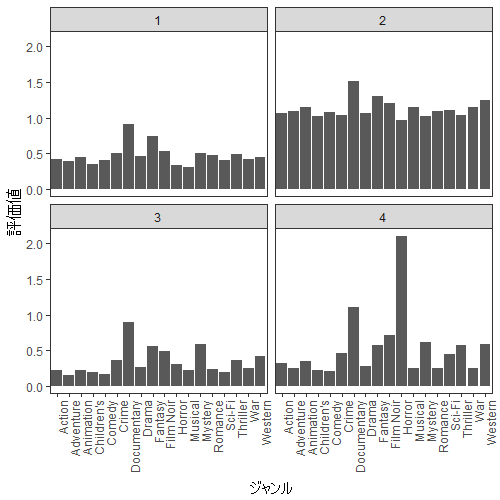
\includegraphics[clip,height= 75mm]{data/cluster_plot.png}
\end{center}
 \vspace{-0.9cm}
\caption{クラスターごとのジャンルへの評価値}
\label{clustergenre}
\end{wrapfigure}

各ユーザの評価値と各映画のジャンル($20$種類)を用いて, ユーザごとに各ジャンルへの総評価値を算出し, 正規化を行った. 各映画には複数のジャンルが対応している. 得られた評価値からクラスターごとのジャンルへの評価値を求めた. 結果を図$\ref{clustergenre}$に示す. クラスター$2$は幅広いジャンルの映画に対して, 高評価を与えているユーザが所属し, クラスター$1,3,4$ではジャンルへの評価値に差が現れた. しかし, ユーザの映画に対する評価値において$0$が非常に多く, 次元圧縮において$0$のデータも特徴として扱われてしまう問題点がある. 実際には$0$のデータはまだ見ていないことを表しており, 特徴として意味がないので, $0$のデータを取り除いて考える必要がある.

%%%%%%%%%%%%%%%%%%%%%%%  section5 まとめ %%%%%%%%%%%%%%%%%%%%%%%%%%%%%
\vspace{-1zh}
\section{まとめ}

本研究では高次元データを$3$次元に圧縮し, クラスタリングを試みたが, 一般化射影正規分布では任意次元の超球面において分布を生成することができるので, 超球面上でのクラスタリングに取り組みたい.

%\newpage
%\addcontentsline{toc}{section}{参考文献} %目次に参考文献を入れる

%必要になる
%\newpage
%\section{付録}

%参考文献を引用する際に必要なコマンド
\bibliographystyle{jplain}
\bibliography{bunken}

%%%%%%%%%%%%%%%%%%%%%%%%%%%%%%%%%%%%%%%%%%%%%%%%%%%%%%%%%%%%%%%%%%%
%%%%%%%%% 参考文献用 bibtexから呼び出すページ %%%%%%%%%%%%%%%%%%%%%%%%%%
\if0
Presnell(1998) \citet{PML}

Wang and Gelfand (2013) \citet{PN1}

% D. Hemandez(2017) \citet{GPN}

Dhillon and Modha(2001) \citet{SKMcluster}

Gopal and Yang(2014) \citet{Gopal}

Neal (2011) \citet{HMC}

Hoffman and Gelman (2013) \citet{NUTS}

L. Maaten and G. Hinton (2008) \citet{tSNE}
\fi

\if0
%%%%%%%% 図の挿入用 %%%%%%%%%%%%%%
\vspace{-0.3cm}
\begin{figure}[H]
\begin{center}
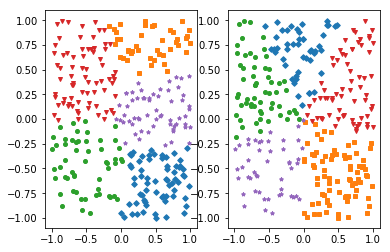
\includegraphics[clip,height= 35mm]{data/kmeans+skmeans.png}
\end{center}
 \vspace{-0.9cm}
\caption{k-meansによるクラスタリング(左), skmeansによるクラスタリング(右)}
\label{skmeans}
\end{figure}

%%%%%%%% 回り込み図の挿入用 %%%%%%%%%%%%%%
\begin{wrapfigure}[10]{r}[5mm]{70mm}
\vspace{-0.6cm}
\centering
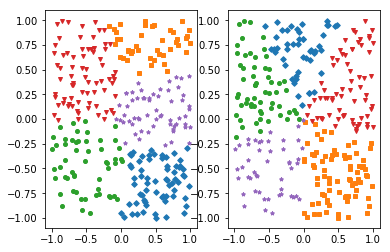
\includegraphics[keepaspectratio,width=70mm]{data/kmeans+skmeans.png}
\vspace{-1cm}
\caption{k-meansによるクラスタリング(左), skmeansによるクラスタリング(右)}
\label{kmeans}
\end{wrapfigure}

%%%%%%%% 複数図の挿入用 %%%%%%%%%%%%%%
\begin{figure}[h]
 \begin{tabular}{c}
\hspace{0.5cm}
 \begin{minipage}{0.5\hsize}
  \begin{center}
   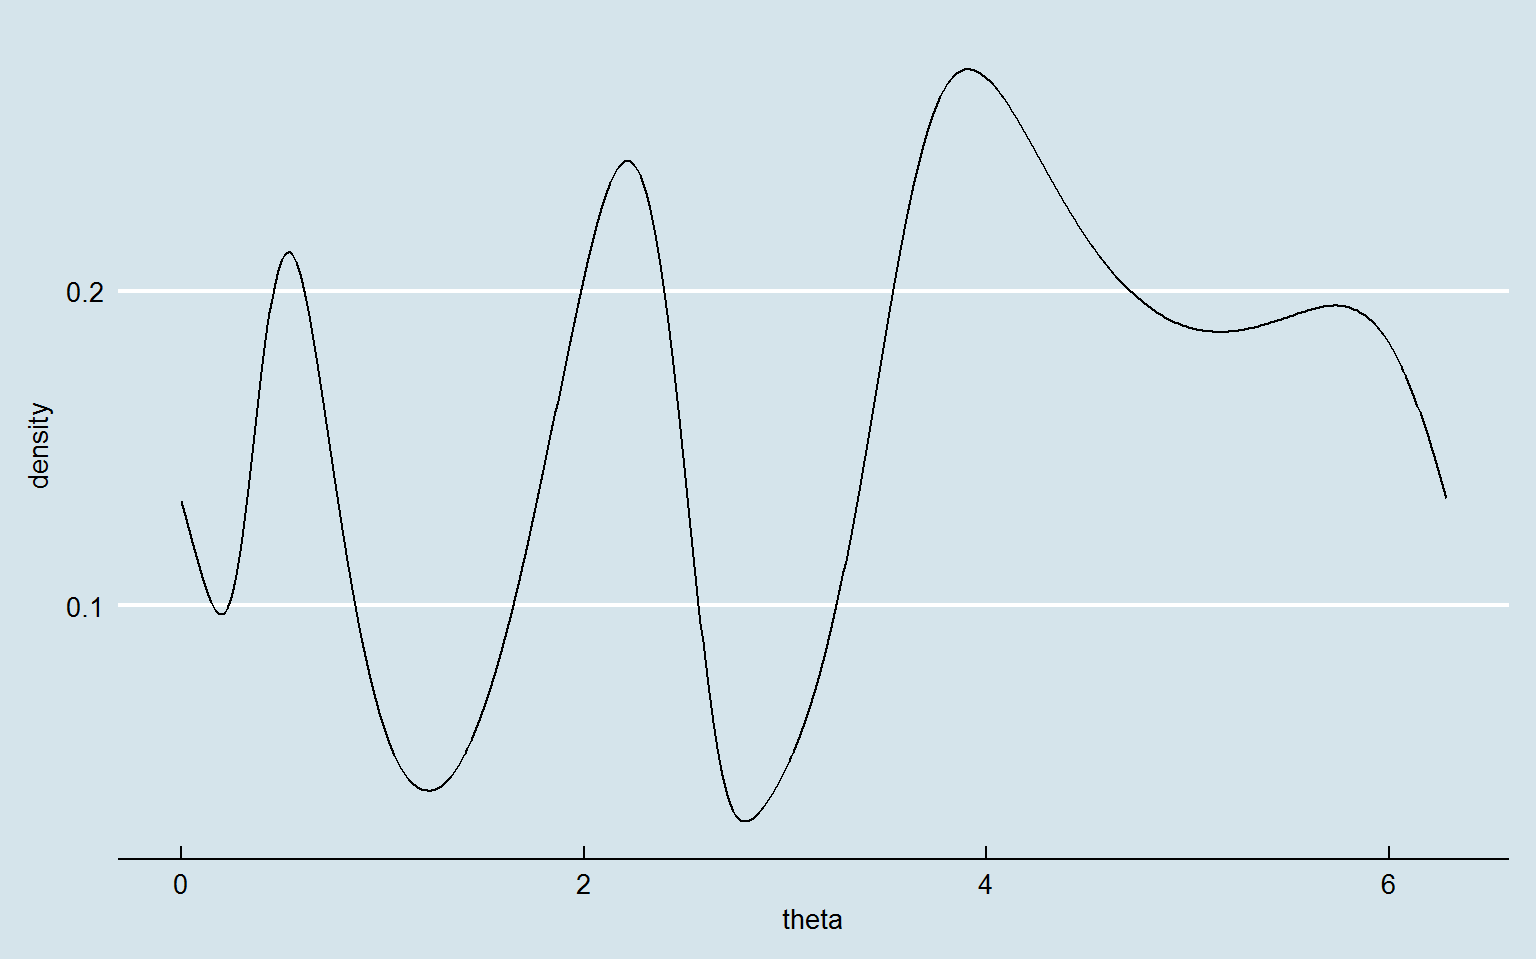
\includegraphics[clip,height= 35mm]{data/mix_pn.png}
  \end{center}
  %\caption{Mixture Projected Normal 分布により推定した混合分布}
  \label{pnmix}
 \end{minipage}
\hspace{-1.0cm}
 \begin{minipage}{0.5\hsize}
  \begin{center}
   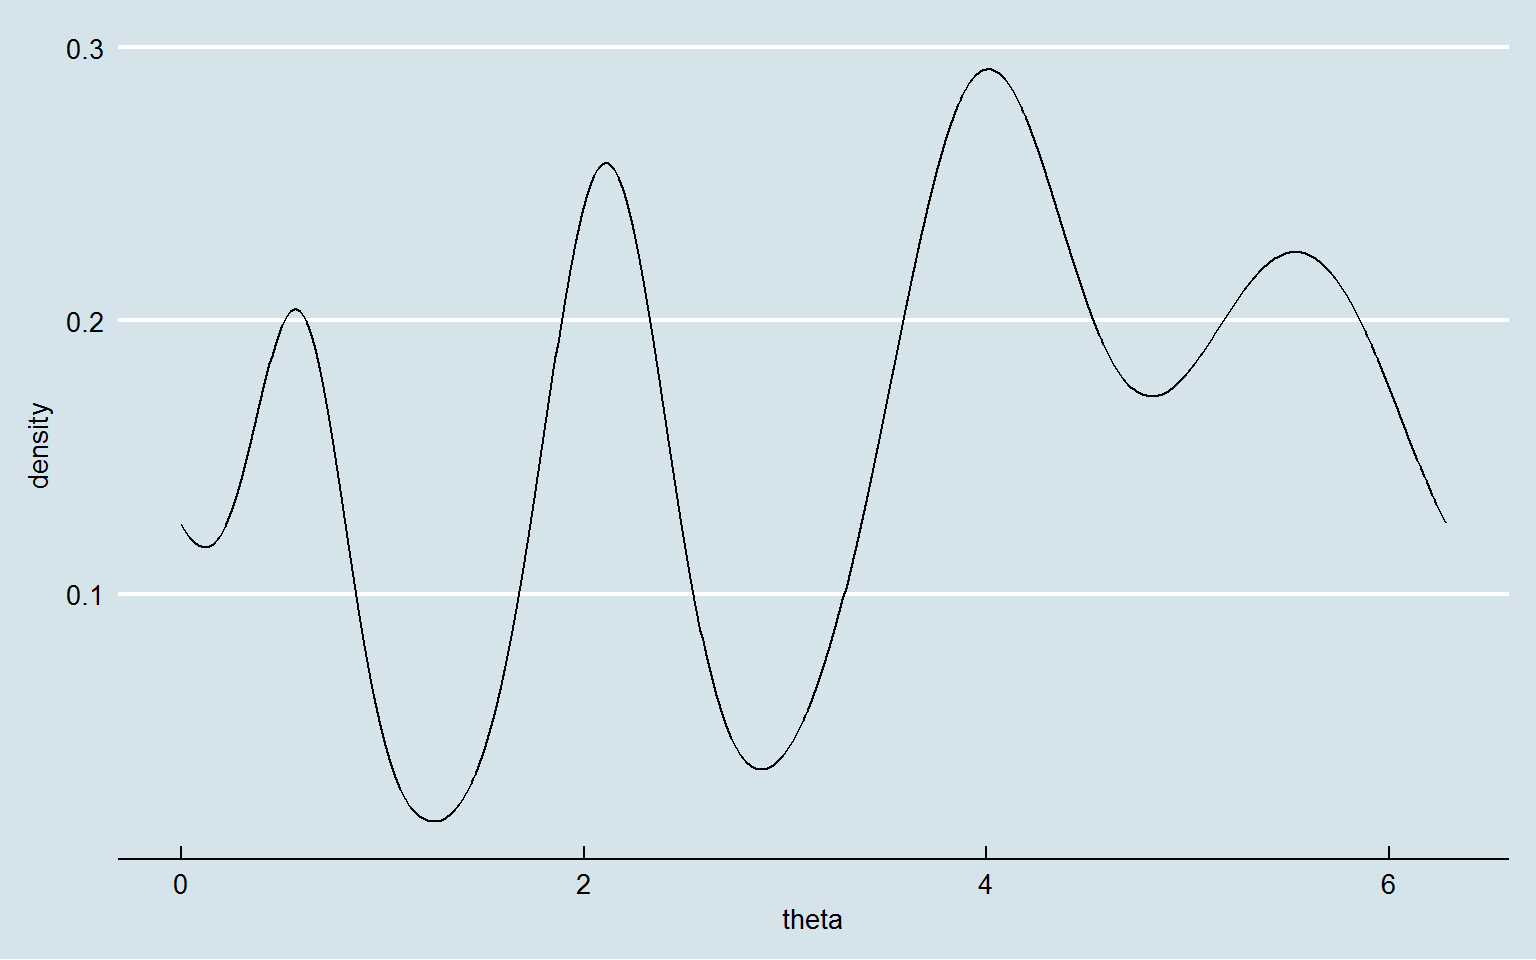
\includegraphics[clip,height= 35mm]{data/mix_von.png}
  \end{center}
 % \caption{Mixture von Mises分布により推定した混合分布}
  \label{vonmix}
 \end{minipage}
  \end{tabular}
\caption{Mixture Projected Normal 分布により推定した混合分布(左), Mixture von Mises分布により推定した混合分布(右)}
\end{figure}
\fi

\if0
%%%%%%%% 複数の表載せる %%%%%%%%%%%%%%
\begin{table}[H]
\caption{PN 分布によるクラスター推定(左), VM 分布によるクラスター推定(右)}
\begin{tabular}{c}
% 1
\hspace{1.5cm}
\begin{minipage}{0.5\hsize}
\begin{center}
%\caption{PN 分布によるクラスター推定}
\begin{tabular}{|c|c|c|c|c|}
\hline
 &  & \multicolumn{3}{|c|}{Predict} \\ \hline
 &  & 1 & 2 & 3 \\ \hline 
 &1 & 38 & 10 & 352 \\ \cline{2-5}
True
 & 2 & 1 & 192 & 7 \\ \cline{2-5}
 & 3 & 0 & 2  & 298 \\ \cline{2-5}
 & 4 & 93 & 0 & 7 \\ 
\hline
 \end{tabular}
 \end{center}
\end{minipage}

% 2
\hspace{-2.5cm}
\begin{minipage}{0.5\hsize}
\begin{center}
%\caption{VM 分布によるクラスター推定}
\begin{tabular}{|c|c|c|c|c|c|}
\hline
 &  & \multicolumn{4}{|c|}{Predict} \\ \hline
 &  & 1 & 2 & 3 & 4 \\ \hline 
 & 1 & 333 & 10 & 39 & 18 \\ \cline{2-6}
True
 & 2 & 7 & 192 & 1 & 0 \\ \cline{2-6}
 & 3 & 298 & 2  & 0 & 0 \\ \cline{2-6}
 & 4 & 0 & 1 & 94 & 5 \\ 
\hline
\end{tabular}
\end{center}
\end{minipage}

\end{tabular}
\end{table}
\fi
\end{document}

%\begin{table}[H]
%\begin{center}
%\caption{条件付確率表(CPT)}   %キャプション
%\label{cpt}   %ラベル
%\begin{tabular}{|c||c|c|c|}   %{}で文字の揃え方を指定
%\hline
% & $Pa(X_{j})=x_{1}$ & \dots & $Pa(X_{j})=x_{m}$
%\\ \hline
%$X_j=y_1$ & $p(y_1|Pa(X_j)=x_1)$ & \dots & $p(y_1|Pa(X_j)=x_m)$
%\\ \hline
%$\vdots$ & $\vdots$ & $\ddots$ & $\vdots$
%\\ \hline
%$X_j=y_n$ & $ p(y_n|Pa(X_j)=x_1)$ & \dots & $p(y_n|Pa(X_j)=x_m)$
%\\ \hline
%\end{tabular}
%\end{center}
%\end{table}
